% Pulsar: методологический отчёт. Сборка: cd docs/report && tectonic report.tex
\documentclass[11pt,a4paper]{article}

\usepackage[left=2.5cm,right=2cm,top=2.2cm,bottom=2.3cm]{geometry}
\usepackage{fontspec}
\setmainfont{cmun}[Extension=.otf,UprightFont=cmunrm,BoldFont=cmunbx,ItalicFont=cmunti,BoldItalicFont=cmunbi]
\setsansfont{cmun}[Extension=.otf,UprightFont=cmunss,BoldFont=cmunsx,ItalicFont=cmunsi,BoldItalicFont=cmunso]
\setmonofont{cmun}[Extension=.otf,UprightFont=cmuntt,BoldFont=cmuntb,ItalicFont=cmunit,BoldItalicFont=cmuntx]
\usepackage[russian]{babel}
\usepackage{amsmath,amssymb}
\usepackage{graphicx}
\usepackage{booktabs,tabularx,array,makecell}
\usepackage{caption}
\usepackage{enumitem}
\usepackage{tikz}
\usetikzlibrary{positioning,arrows.meta}
\usepackage{xcolor}
\definecolor{linkgreen}{HTML}{148F2B}
\usepackage[hyphens]{url}
\usepackage[colorlinks=true,linkcolor=linkgreen,citecolor=linkgreen,urlcolor=linkgreen,pdfauthor={Екатерина Алексанян},pdftitle={Типы локальных экономик России по безналичным тратам}]{hyperref}

\graphicspath{{../figures/}}
\captionsetup{font=small,labelfont=bf,labelsep=period}
\captionsetup[table]{position=top,skip=4pt}
\setlist{itemsep=2pt,topsep=4pt}
\newcolumntype{Y}{>{\raggedright\arraybackslash\hspace{0pt}}X}
\newcommand{\code}[1]{\path{#1}}
\newcommand{\rub}{руб.}
\newcommand{\Kt}{K}
\urlstyle{tt}
\setlength{\emergencystretch}{2em}
\renewcommand{\arraystretch}{1.15}

\title{Типы локальных экономик России по безналичным тратам:\\ динамическая атрибутированная сеть муниципальных образований}
\author{Екатерина Алексанян\\[2pt]
\small МГУ имени М.\,В.~Ломоносова, факультет ВМК\\[6pt]
\small Проект Pulsar. Конкурс СберИндекса 2026, трек <<Кластеризация>>}
\date{9 октября 2026}

\begin{document}
\maketitle

\begin{abstract}
\noindent\textit{Вопрос.} Какие типы локальных экономик видны в безналичных тратах жителей 2\,016 муниципальных образований (МО) за 2023--2024~гг., как эти территории связаны между собой и как группы меняются во времени?

\smallskip\noindent\textit{Метод.} (1) Семь признаков на МО-месяц: состав трат (CLR долей шести категорий) и уровень трат относительно страны. Признаков Росстата в модели нет, они оставлены для проверки. (2) Сеть близости из трёх слоёв с разными источниками информации (поведение: сходство профилей; со-движение: лаговые корреляции приростов; география: дорожные расстояния), слитых диффузией SNF; граф месяца $t$ использует только данные $\le t$. (3) Семь методов на одинаковых входах, от k-means до KEFRiN и temporal Leiden, и десять индексов качества, сверенных с библиотекой Pattern. Нулевые модели и парный бутстрэп показывают, какие различия между методами значимы. (4) Сквозные типы и подтверждённые переходы (новый тип держится $\ge 3$ месяцев при бутстрэп-уверенности $\ge 0{,}7$), индекс Шоррокса, события жизненного цикла; онлайн-проверка: центры 2023~г. классифицируют 2024~г. без пересчёта. (5) Интерпретация: профили по Миркину \cite{mirkin-book}, дерево правил в рублях и процентах, внешняя проверка зарплатами, структурой занятости и населением Росстата.

\smallskip\noindent\textit{Результаты.} Шесть устойчивых типов локальных экономик: \textbf{мегаполисы и столичные районы} (16\,\% МО; траты 186\,\% от медианы страны, самый устойчивый тип), \textbf{промышленные города и пригороды} (20\,\%), \textbf{малые города и райцентры} (22\,\%), \textbf{аграрные районы на трассах} (16\,\%; самый подвижный), \textbf{сельская периферия} (21\,\%; траты 82\,\% медианы) и \textbf{Север и ресурсные территории} (6\,\%; дорогая логистика, вдвое меньшая доля маркетплейсов). Типы объясняют 61\,\% разброса зарплат и 48\,\% разброса населения по данным Росстата, не участвовавшим в обучении модели. За два года 68\,\% МО не сменили тип ни разу; индекс Шоррокса по подтверждённым переходам 0,02 в месяц и 0,17 за год (декабрь 2023 $\to$ декабрь 2024); ни один тип не возник и не исчез. Главный сдвиг периода: доля маркетплейсов удвоилась во всех типах, Север отстаёт. Шоки (паводок в Орске) видны как сдвиг структуры трат и падение уверенности типа, но тип не меняется. Апрельский разрыв 2023~г. вызван сменой методики, и правило подтверждения его отфильтровывает.

\smallskip\noindent\textit{Воспроизводимость.} Все числа воспроизводятся командой \texttt{make all} (время прогона в приложении~\ref{app:runtime}). Данные: Лаборатория СберИндекс, CC BY-SA 4.0. Репозиторий: \url{https://github.com/estnafinema0/sberindex-pulsar}; лендинг: \url{https://estnafinema0.github.io/sberindex-pulsar/}.
\end{abstract}

\tableofcontents
\bigskip

\section*{Схема работы}
\addcontentsline{toc}{section}{Схема работы}

Конвейер показан на рис.~\ref{fig:pipeline}; критерии и расположение кода в репозитории представлены в табл.~\ref{tab:criteria}.

\begin{figure}[htbp]
\centering
\begin{tikzpicture}[
  box/.style={draw, rounded corners=2pt, align=center, font=\small, minimum height=9mm, inner sep=4pt, text width=#1},
  box/.default=3.3cm,
  arr/.style={-{Stealth[length=2.2mm]}, thick},
  node distance=6mm and 7mm]
\node[box] (data) {Траты\\ МО $\times$ месяц $\times$ категория};
\node[box, right=of data] (feat) {Признаки $X_t$\\ (CLR, уровень)};
\node[box, right=of feat] (graph) {3 слоя сети $\to$ SNF,\\ граф $A_t$};
\node[box, below=9mm of graph] (meth) {7 методов,\\ $K\in 4..10$};
\node[box, below=of meth] (icvi) {10 ICVI, нулевые модели, бутстрэп $\to$ метод и $K$};
\node[box, left=of icvi] (types) {Типы МО};
\node[box, left=of types] (ext) {Внешняя проверка: Росстат, тип МО, доступность рынков};
\node[box, below=of types] (dyn) {Подтверждённые переходы, out-of-time};
\node[box, right=of dyn] (out) {Карта, паспорта типов, кейсы};
\draw[arr] (data) -- (feat);
\draw[arr] (feat) -- (graph);
\draw[arr] (graph) -- (meth);
\draw[arr] (feat.south) |- (meth.west);
\draw[arr] (meth) -- (icvi);
\draw[arr] (icvi) -- (types);
\draw[arr] (types) -- (ext);
\draw[arr] (types) -- (dyn);
\draw[arr] (dyn) -- (out);
\end{tikzpicture}
\caption{Схема работы}
\label{fig:pipeline}
\end{figure}

\begin{table}[htbp]
\centering\small
\captionsetup{labelsep=none}\caption{}
\label{tab:criteria}
\begin{tabularx}{\textwidth}{>{\raggedright\arraybackslash\hspace{0pt}}p{3.2cm}>{\raggedright\arraybackslash\hspace{0pt}}p{2.3cm}YY}
\toprule
Критерий & Раздел & Код & Тест \\
\midrule
Методология & \ref{sec:data}--\ref{sec:network} & \code{src/pulsar/features.py}, \code{graphs.py} & \code{tests/test_features.py}, \code{test_graphs.py} \\
Сеть и атрибуты & \ref{sec:network}, прил.~\ref{app:ablation} & \code{graphs.py}, \code{build_graphs.py} & \code{test_graphs.py} \\
Сравнение методов & \ref{sec:methods} & \code{methods.py}, \code{run_cluster.py}, \code{compare.py} & \code{test_methods.py}, \code{test_evaluate.py} \\
ICVI & \ref{sec:methods}, прил.~\ref{app:icvi} & \code{icvi.py}, \code{evaluate.py} & \code{test_icvi.py} (сверка с Pattern) \\
Интерпретация, воспроизводимость & \ref{sec:types}--\ref{sec:dynamics}, README & \code{dynamics.py}, \code{interpret.py} & \code{test_interpret.py} \\
Визуализация & лендинг & \code{site/} & -- \\
\bottomrule
\end{tabularx}
\end{table}

%=====================================================================
\section{Данные и признаки}\label{sec:data}

\subsection{Данные}\label{sec:data-raw}
Основные данные – оценки средних безналичных трат жителя МО в месяц (\rub) по шести категориям (<<Все категории>>, Продовольствие, Здоровье, Маркетплейсы, Общественное питание, Транспорт), 303\,126 строк, 2\,190 МО, 24 месяца (01.2023--12.2024). МО попадает в месяц, только если оценка прошла порог качества, поэтому панель несбалансирована. Полная история есть у 2\,016 МО, они образуют обучающую панель; остальные 174 МО классифицируются по ближайшему центру типа и показаны на карте с пометкой. В данных нет восьми приграничных регионов (Белгородская, Брянская, Воронежская, Курская, Ростовская области, Краснодарский край, Крым, Севастополь); 247 МО относятся к внутригородским территориям Москвы и Петербурга.

Дополнительно использованы расстояния между центрами МО по автодорогам (5,9~млн пар; у 148 пар <<город / одноимённый район>> расстояние нулевое из-за общего центра, заменяем на 5~км), индекс доступности рынков, справочник <<Границы и изменения МО>> (типы, статусы, регионы, полигоны) и, только для внешней проверки, Росстат (БДМО): зарплаты и численность работников по разделам ОКВЭД2, население (см. \code{docs/external_data.md}).

В данных есть два системных эффекта: (1) в апреле 2023~г. у 30--38\,\% МО синхронно падают оценки по <<Здоровью>> ($-17$\,\% медианно) и <<Общепиту>> ($-18$\,\%). (2) Сезонность сильная (декабрь $+19$\,\% к ноябрю, январь $-23$\,\%). Оба эффекта снимаются центрированием внутри месяца (п.~\ref{sec:features}) и правилом подтверждения перехода (п.~\ref{sec:transitions}).

\subsection{Признаки месяца}\label{sec:features}
Для МО $i$ в месяце $t$ берём доли шести компонент итога $s_{ic}$ (пять категорий и <<Прочее>> $=1-\sum_c s_{ic}$; <<Прочее>> в медиане составляет 28\,\% итога, без него композиция неполна и CLR некорректен) и сам итог $y_{it}$.

\begin{itemize}
\item CLR долей \cite{aitchison}:
\begin{equation}\label{eq:clr}
\mathrm{clr}_{ic} = \ln s_{ic} - \frac16\sum_{c'}\ln s_{ic'}.
\end{equation}
Доли образуют композиционные данные, и евклидово расстояние между ними бессмысленно; CLR переводит их в пространство, где k-means, Ward и ядра корректны. Шесть компонент, сумма CLR равна нулю (ранг~5).
\item Относительный уровень:
\begin{equation}\label{eq:level}
\ell_{it} = \ln\bigl(y_{it} / \mathrm{med}_j\, y_{jt}\bigr).
\end{equation}
Один признак <<богатства>> территории; деление на медиану страны в том же месяце убирает общий сезон и инфляцию, остаётся положение МО относительно страны.
\item Причинное сглаживание: среднее за $t-2..t$. Используется для уменьшения шума оценок и не использует данные о будущем (признаки месяца $t$ известны в месяце $t$).
\item Стандартизация внутри месяца: $z$-оценка по МО. Признаки сопоставимы между месяцами, сезон не влияет на расстояния; все семь признаков входят с равным весом.
\end{itemize}

Итог: $X_t \in \mathbb{R}^{2016\times 7}$ для каждого из 24 месяцев. Признаки Росстата в $X_t$ не входят, так как используются для внешней проверки.

%=====================================================================
\section{Сеть: правило ребра и его влияние}\label{sec:network}

\subsection{Три слоя и формулы}\label{sec:layers}
Жюри предлагает три семейства близости: по схожести векторов трат, по взаимному опережению (лаговые корреляции, DTW) и по расстояниям между регионами. Мы строим по слою на каждое семейство так, чтобы слои несли разную информацию, и затем сливаем их. Граф месяца $t$ использует только данные $\le t$.

\paragraph{Слой 1, поведение (сходство профилей).} $d_{ij}=\|x_i-x_j\|$ в пространстве признаков месяца; локальный масштаб $\sigma_i$ равен расстоянию до 7-го соседа \cite{zelnik}; вес
\begin{equation}\label{eq:selftune}
w_{ij}=\exp\!\bigl(-d_{ij}^2/(\sigma_i\sigma_j)\bigr);
\end{equation}
ребро остаётся, если $i\in\mathrm{kNN}_{10}(j)$ и $j\in\mathrm{kNN}_{10}(i)$ (взаимный kNN режет <<хабы>> плотных зон); добавляются рёбра минимального остовного дерева, поэтому граф связный, без изолятов. Самонастраивающееся ядро нужно потому, что плотность МО в признаковом пространстве различается на порядок (сёла и столичные районы): один глобальный $\sigma$ либо склеивает первых, либо рвёт вторых.

\paragraph{Слой 2, со-движение (лаговые корреляции).} $Z$: стандартизованные лог-приросты итоговых трат за прошлые $W=12$ месяцев за вычетом медианы страны (общий тренд убран). При $N=2016\gg W$ выборочная корреляция вырождена, поэтому используется оценка с усадкой \cite{ledoit}
\begin{equation}\label{eq:lw}
\Sigma_{LW}=(1-\delta)S+\delta\mu I,\qquad \rho_{ij}=\Sigma_{ij}/\sqrt{\Sigma_{ii}\Sigma_{jj}};
\end{equation}
для лага $L=1$ считается кросс-корреляция сдвинутых рядов, берём $\max_L\rho^{(L)}_{ij}$, отрицательные обнуляем, оставляем 10 сильнейших взаимно. В первые три месяца окна нет, слой пустой и в слиянии пропускается. DTW в работе не используется: на рядах длиной 12--24 точки выравнивание по времени мало отличается от сдвига на $\pm1$ месяц, который уже учитывает лаговая корреляция.

\paragraph{Слой 3, география (расстояния).} $w_{ij}=\exp(-D_{ij}/200\,\text{км})$ по автодорогам (ж/д -- в качестве запасного варианта, большой круг $\times\,1{,}3$ для 1,2\,\% пар без дорог), 10 ближайших, симметризация по max. 200~км примерно соответствуют радиусу <<регионального рынка>>. Этот слой не зависит от трат и проверяет, добавляет ли пространство что-то к поведению.

\paragraph{Слияние через SNF \cite{wang}.} Для каждого слоя строятся полная нормированная матрица $P^{(v)}$ и локальное ядро $S^{(v)}$ по 10 соседям; итерации
\begin{equation}\label{eq:snf}
P^{(v)}\leftarrow S^{(v)}\,\overline{P^{(-v)}}\,S^{(v)\top},\qquad t=10;
\end{equation}
итого: среднее $P^{(v)}$, взаимный kNN$_{10}$ и максимальное остовное дерево. SNF выбран вместо среднего весов, потому что диффузия усиливает рёбра, поддержанные несколькими слоями, и подавляет шум одного слоя. Вариант со средним весов реализован в коде (\texttt{fusion.method: mean}), но в этой работе не сравнивался.

Все гиперпараметры лежат в \code{configs/graph.yaml}.

\subsection{Что меняет правило ребра}\label{sec:edge-rule}

\begin{table}[htbp]
\centering\small
\caption{Структура сети по слоям (медианы по 24 месяцам).}
\label{tab:network}
\footnotesize\setlength{\tabcolsep}{3pt}
\begin{tabularx}{\textwidth}{>{\raggedright\arraybackslash\hspace{0pt}}p{1.9cm}*{8}{>{\centering\arraybackslash\hspace{0pt}}X}}
\toprule
Слой & ср.\ степень & компонент & изолятов & ассор\-та\-тив\-ность & кластер.\ коэф. & алгебр.\ связность & негладкость, $x^{\!\top}\!Lx\,/$ $x^{\!\top}\!x$ & ср.\ длина ребра в признаках \\
\midrule
поведение & 6.3 & 1 & 0.0\,\% & 0.42 & 0.32 & 0.002 & 0.10 & 0.68 \\
со-движение & 5.8 & 20 & 0.8\,\% & 0.35 & 0.19 & 0.004 & 0.61 & 2.51 \\
география & 12.5 & 1 & 0.0\,\% & 0.16 & 0.59 & 0.000 & 0.43 & 2.09 \\
слитый (SNF) & 8.5 & 1 & 0.0\,\% & 0.10 & 0.19 & 0.025 & 0.27 & 1.58 \\
\bottomrule
\end{tabularx}
\end{table}

Слои почти не пересекаются по рёбрам (Жаккар множеств рёбер между любыми двумя слоями 0,015--0,035 в 2024-06), то есть несут разную информацию (табл.~\ref{tab:network}, рис.~\ref{fig:layers}). Географический слой самый <<кластеризованный>> (коэффициент 0,59: соседи соседей тоже соседи) и самый гладкий по степеням. Поведенческий слой самый ассортативный, и рёбра у него самые короткие в признаковом пространстве (0,68\,$\sigma$ против 2,1 у географии), что ожидаемо: он построен из тех же признаков. Слой со-движения появляется с четвёртого месяца (нужно окно $\ge 3$) и имеет изоляты: у части МО приросты ни с кем значимо не коррелируют. Слитый граф связный, без изолятов, со средней степенью 8,5 и промежуточной гладкостью признаков (0,27). Он сохраняет компактность поведения и добавляет рёбра географии и со-движения.

\begin{figure}[htbp]
\centering
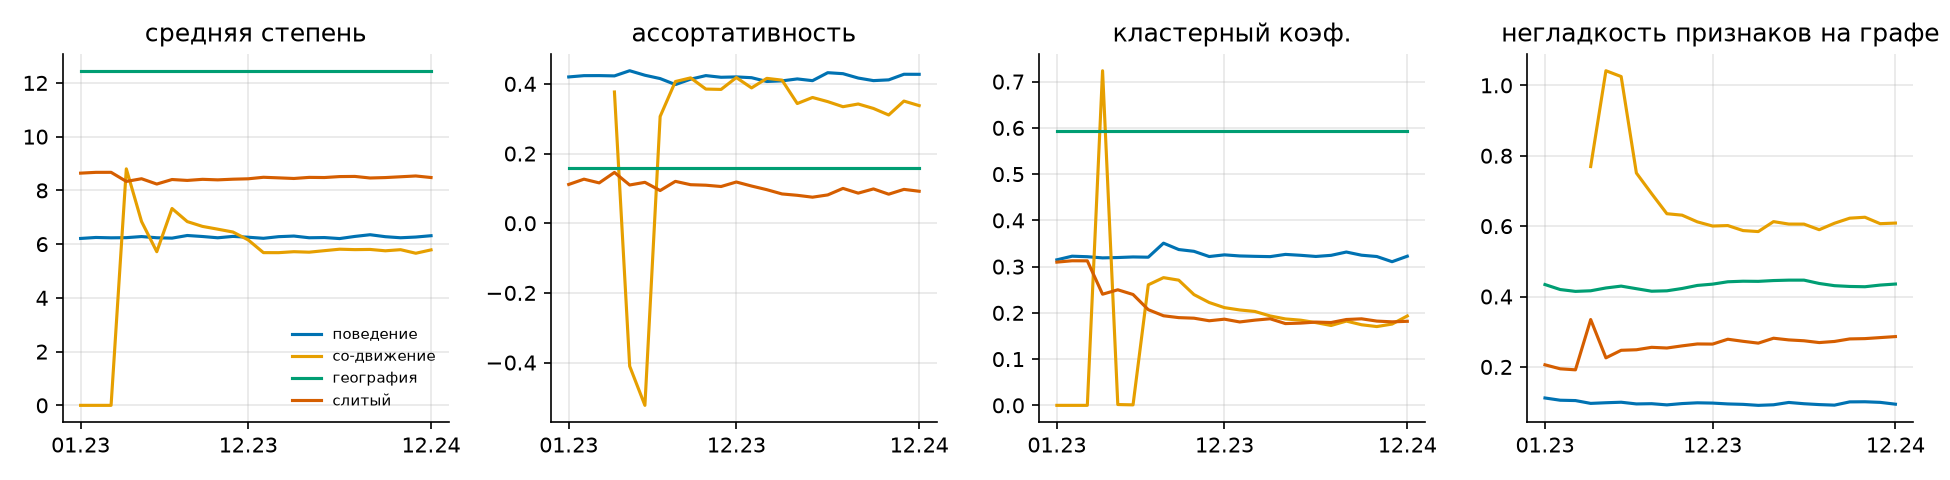
\includegraphics[width=\textwidth]{layers.png}
\caption{Характеристики слоёв сети по месяцам: средняя степень, ассортативность, кластерный коэффициент, негладкость признаков на графе.}
\label{fig:layers}
\end{figure}

\begin{table}[htbp]
\centering\small
\caption{ICVI при $K=6$ для одного метода на разных слоях (медианы по месяцам).}
\label{tab:layer-icvi}
\begin{tabular}{llrrrrr}
\toprule
Слой & Метод & SW & AVI & AVU & MQ$=Q$ & ANUI \\
\midrule
поведение & KEFRiN (сбал.) & 0.217 & 0.887 & 0.524 & 0.701 & 0.606 \\
 & Leiden & 0.159 & 0.948 & 0.433 & 0.711 & 0.670 \\
 & Spectral & 0.164 & 0.936 & 0.526 & 0.632 & 0.628 \\
\addlinespace
со-движение & KEFRiN (сбал.) & 0.216 & 0.414 & 0.505 & 0.221 & 0.342 \\
 & Leiden & $-0.057$ & 0.906 & 0.460 & 0.598 & 0.625 \\
 & Spectral & $-0.046$ & 0.959 & 0.367 & 0.320 & 0.700 \\
\addlinespace
география & KEFRiN (сбал.) & 0.214 & 0.528 & 0.461 & 0.323 & 0.424 \\
 & Leiden & $-0.042$ & 0.993 & 0.363 & 0.714 & 0.729 \\
 & Spectral & $-0.006$ & 0.960 & 0.415 & 0.667 & 0.686 \\
\addlinespace
слитый (SNF) & KEFRiN (сбал.) & 0.218 & 0.684 & 0.504 & 0.495 & 0.509 \\
 & Leiden & 0.086 & 0.849 & 0.444 & 0.568 & 0.617 \\
 & Spectral & 0.060 & 0.839 & 0.446 & 0.445 & 0.610 \\
\bottomrule
\end{tabular}
\end{table}

\begin{table}[htbp]
\centering\small
\caption{Зависимость типологии от слоя: ARI между разбиениями одного метода на разных слоях (медиана по месяцам).}
\label{tab:layer-ari}
\begin{tabularx}{\textwidth}{>{\raggedright\arraybackslash\hspace{0pt}}p{2.8cm}*{4}{>{\centering\arraybackslash\hspace{0pt}}X}}
\toprule
Метод & поведение $\sim$ со-движение & поведение $\sim$ география & со-движение $\sim$ география & слой $\sim$ слитый (медиана трёх) \\
\midrule
KEFRiN (сбал.) & 0.93 & 0.87 & 0.88 & 0.90 \\
Leiden & 0.12 & 0.15 & 0.09 & 0.23 \\
Spectral & 0.19 & 0.14 & 0.04 & 0.33 \\
\bottomrule
\end{tabularx}
\end{table}

Выводы по табл.~\ref{tab:layer-icvi} и~\ref{tab:layer-ari}. (1) Для чисто сетевых методов правило ребра определяет модель целиком. Leiden на географии даёт AVI 0,99 и $Q$ 0,71, но SW $<0$: он выделяет региональные блоки, которые с типами экономики не совпадают. На со-движении SW тоже отрицательный. Типологии этих методов на разных слоях почти не связаны (ARI 0,1--0,3). (2) У KEFRiN с уравновешенными вкладами слой меняет сетевые индексы вдвое ($Q$ от 0,22 на со-движении до 0,70 на поведении), но типология устойчива (ARI 0,87--0,93): структура трат задаёт типы, сеть уточняет границы между ними. (3) Слитый граф выбран основным, хотя на поведенческом слое $Q$ выше: только слитый граф содержит информацию всех трёх семейств близости из критерия жюри, связен и даёт устойчивую типологию. $Q$ при этом равен 0,50 против 0,70 у <<автокоррелированного>> поведенческого слоя, построенного из тех же признаков, что и атрибуты.

%=====================================================================
\section{Методы и их сравнение}\label{sec:methods}

\subsection{Семь вариантов на одних входах}\label{sec:seven}
Все методы получают одинаковые $X_t$ и $A_t$ (слитый граф), одинаковые $K$ и seed. Порядок в табл.~\ref{tab:methods}: от <<только признаки>> к <<только сеть>> и <<оба>>. Критерий Leiden \cite{traag} и KEFRiN \cite{shalileh-mirkin-entropy}:
\begin{gather}
\max_{g}\; Q_\gamma=\frac1{2m}\sum_{ij}\Bigl(A_{ij}-\gamma\frac{k_ik_j}{2m}\Bigr)\delta(g_i,g_j), \label{eq:modularity}\\
F=\rho\|Y-SC\|^2+\xi\|P-S\Lambda\|^2,\qquad P=A-\frac{kk^\top}{2m}. \label{eq:kefrin}
\end{gather}

\begin{table}[htbp]
\centering\small
\caption{Методы сравнения.}
\label{tab:methods}
\begin{tabularx}{\textwidth}{>{\raggedright\arraybackslash\hspace{0pt}}p{2.2cm}>{\raggedright\arraybackslash\hspace{0pt}}p{5.0cm}>{\raggedright\arraybackslash\hspace{0pt}}p{1.8cm}Y}
\toprule
Метод & Критерий & Входы & Комментарий \\
\midrule
k-means & $\min\sum_k\sum_{i\in S_k}\|x_i-c_k\|^2$ & $X_t$ & базовая линия по признакам \\
Ward & то же, агломеративно & $X_t$ & детерминированная база, иерархия \\
Spectral & $K$ собственных векторов нормированного лапласиана $A_t$, затем k-means & $A_t$ & <<чистая>> сеть, релаксация нормированного разреза \\
Leiden & $\max Q_\gamma$ \eqref{eq:modularity}, $\gamma$ подбирается под $K$ & $A_t$ & эталон сетевых методов \cite{traag} \\
temporal Leiden & мультислойная модулярность \cite{mucha}: $+\,\omega\,\delta_{ij}$ между соседними месяцами, $\omega=0{,}25$ & $A_1..A_{24}$ & единственный метод, где типы сквозные по построению \\
KEFRiN & $F$ \eqref{eq:kefrin} \cite{shalileh-mirkin-entropy}, $\rho=\xi=1$ & $X_t$, $A_t$ & метод жюри, реализован по формулам \\
KEFRiN (сбаланс.) & то же, $\xi\leftarrow\xi\,\|Y\|^2/\|P\|^2$ & $X_t$, $A_t$ & при $\rho=\xi=1$ на разреженной сети $\|P\|^2\approx 2\,\%$ от $\|Y\|^2$ и сеть почти не влияет; балансировка уравнивает вклады \\
\bottomrule
\end{tabularx}
\end{table}

KEFRiN: чередование <<объект $\to$ ближайший центр по сумме двух расстояний>> и <<центры $=$ средние>>, инициализация K-Means++, 5 стартов, лучший по $F$; каждый шаг не увеличивает $F$ (тест). Temporal Leiden: разрешение $\gamma$ подбирается бисекцией так, чтобы медианное по срезам число сообществ размером $\ge 5$ равнялось $K$; мелкие сообщества присоединяются к соседям. Для помесячных методов сквозные номера получаются венгерским сопоставлением по Жаккару между соседними месяцами (\code{src/pulsar/align.py}).

\subsection{Панель ICVI и её подводные камни}\label{sec:icvi}
Считаем шесть индексов из Положения (SW \cite{rousseeuw}, CH \cite{calinski}, S\_Dbw \cite{halkidi} по признакам; AVI, AVU, MQ по сети) и дополняем их ANUI, DBI \cite{davies}, CH/$N$ и плотностной модулярностью, следуя панели из работ жюри \cite{shalileh-doklady,shalileh-eswa}. Все реализации свои (\code{src/pulsar/icvi.py}). Сетевые индексы численно совпадают с библиотекой Pattern Лаборатории СберИндекс до $10^{-9}$ (тест \code{test_matches_pattern_library}), S\_Dbw совпадает с пакетом \code{s-dbw} в его соглашениях и отдельно сверен со статьёй \cite{halkidi}.

Обозначения: $S_{ab}$~-- суммарный вес рёбер между кластерами $a$ и $b$ (внутренний считается дважды), $\mathrm{out}_a=\sum_{b\ne a}S_{ab}$.
\begin{align}
\mathrm{AVI} &= \frac1K\sum_a \frac{S_{aa}}{S_{aa}+\mathrm{out}_a}, \label{eq:avi}\\
\mathrm{AVU} &= \frac1K\sum_a\sum_{b\ne a}\frac{S_{ab}}{\mathrm{out}_a+\mathrm{out}_b-S_{ab}}, \label{eq:avu}\\
\mathrm{ANUI} &= 1/(\mathrm{AVU}+1/\mathrm{AVI}). \label{eq:anui}
\end{align}
\begin{itemize}
\item AVI \eqref{eq:avi}: средняя изолируемость \cite{biswas}, больше лучше. У случайного разбиения $\approx 1/K$ (тест).
\item AVU \eqref{eq:avu}: средняя объединяемость, меньше лучше. Вырожден при малых $K$: при $K=2$ тождественно равен 1, при $K=3$ равен $2/3$ для любого разбиения с непустым разрезом (доказательство в прил.~\ref{app:icvi}, проверено тестом); у случайного разбиения $\approx (K-1)/(2K-3)$ ($0{,}60$ при $K=4$, $0{,}55$ при $K=7$). AVU инвариантен к масштабу внутренних весов и видит только форму разреза. Поэтому сетка $K$ начинается с 4, а AVU сравнивается через $z$-оценки.
\item ANUI \eqref{eq:anui}: сводный индекс Pattern \cite{biswas,howie}; набор индексов для атрибутированных сетей следует \cite{shalileh-profiling}.
\item MQ. В работах жюри MQ означает модулярность Ньюмана--Гирвана $Q$ \cite{newman}, её и считаем как MQ. Для полноты в приложении даны MQ Манкоридиса \cite{mancoridis} и TurboMQ \cite{mitchell}; на неориентированном графе $\mathrm{TurboMQ}\equiv K\cdot\mathrm{AVI}$ (прил.~\ref{app:icvi}), то есть новой информации он не несёт.
\item SW, CH, DBI считаются через sklearn; CH растёт $\sim N$, поэтому рядом даём CH/$N$. У S\_Dbw меньше лучше.
\end{itemize}

Два вида нулевых моделей: (1) перестановка меток при сохранении размеров кластеров даёт $z$-оценку и $p$ каждого индекса (сколько структуры в разбиении по сравнению со случайным разбиением тех же размеров); (2) configuration model переставляет рёбра с сохранением степеней при фиксированных метках (сколько в сетевых индексах объясняется одними степенями). Значимость различий между методами оцениваем парным бутстрэпом по 24 месяцам: ДИ разности средних индексов и доля бутстрэп-выборок, где метод лучший.

\subsection{Результаты}\label{sec:results}

\begin{table}[htbp]
\centering\small
\caption{Индексы при $K=6$: медиана по 24 месяцам (для SW $\pm$ межквартильный размах). Temporal Leiden считался на сетке $K\in\{4,6,8\}$.}
\label{tab:icvi-k6}
\setlength{\tabcolsep}{4pt}
\begin{tabular}{lrrrrrrr}
\toprule
Метод & SW $\uparrow$ & CH $\uparrow$ & S\_Dbw $\downarrow$ & AVI $\uparrow$ & AVU $\downarrow$ & MQ$=Q$ $\uparrow$ & ANUI $\uparrow$ \\
\midrule
k-means & 0{,}218 $\pm$ 0{,}005 & 646 & 0{,}87 & 0{,}665 & 0{,}517 & 0{,}481 & 0{,}495 \\
Ward & 0{,}160 $\pm$ 0{,}026 & 518 & 0{,}84 & 0{,}704 & 0{,}486 & 0{,}508 & 0{,}525 \\
Spectral & 0{,}060 $\pm$ 0{,}054 & 214 & 0{,}81 & 0{,}839 & 0{,}446 & 0{,}445 & 0{,}610 \\
Leiden & 0{,}086 $\pm$ 0{,}049 & 293 & 0{,}73 & 0{,}849 & 0{,}444 & 0{,}568 & 0{,}617 \\
KEFRiN ($\rho=\xi=1$) & 0{,}218 $\pm$ 0{,}006 & 646 & 0{,}84 & 0{,}665 & 0{,}516 & 0{,}483 & 0{,}496 \\
KEFRiN (сбаланс.) & 0{,}218 $\pm$ 0{,}006 & 645 & 0{,}88 & 0{,}684 & 0{,}504 & 0{,}495 & 0{,}509 \\
temporal Leiden ($\omega=0{,}25$) & 0{,}108 & 290 & 0{,}73 & 0{,}830 & 0{,}406 & 0{,}536 & 0{,}622 \\
\bottomrule
\end{tabular}
\end{table}

Случайные уровни при $K=6$: AVI $\approx 0{,}167$, AVU $\approx 0{,}556$. Картина устойчива по месяцам (IQR SW $\le 0{,}02$) и по $K$ (рис.~\ref{fig:kcurves}):
\begin{itemize}
\item Методы по признакам (k-means, Ward, KEFRiN) выигрывают по SW, CH, S\_Dbw; методы по сети (Leiden, Spectral) выигрывают по AVI, AVU, MQ и ANUI (табл.~\ref{tab:icvi-k6}). Расхождение образует фронт Парето <<признаки / сеть>> (рис.~\ref{fig:pareto}) и от реализаций не зависит. Leiden при $K=6$ даёт $Q=0{,}57$, но SW $=0{,}09$: его сообщества почти не различаются по составу трат и потому не читаются как типы экономики.
\item AVU у методов по признакам идёт параллельно случайному уровню (пунктир на рис.~\ref{fig:kcurves}). Индекс падает с ростом $K$ из-за смены базового уровня, качество разбиения при этом не растёт. Поэтому AVU мы сравниваем только через $z$-оценки.
\item KEFRiN в исходной параметризации ($\rho=\xi=1$) почти совпадает с k-means (ARI 0,97 по медиане месяцев): при разреженной сети $\|P\|_F^2$ составляет 2\,\% от $\|Y\|_F^2$, и сетевое слагаемое не влияет на решение. Сбалансированный вариант ($\xi_{\text{eff}} \approx 43$) сохраняет SW k-means и поднимает AVI, MQ и ANUI. Из всех методов только он сдвигает решение к сети без потери читаемости профилей.
\end{itemize}

\begin{figure}[htbp]
\centering
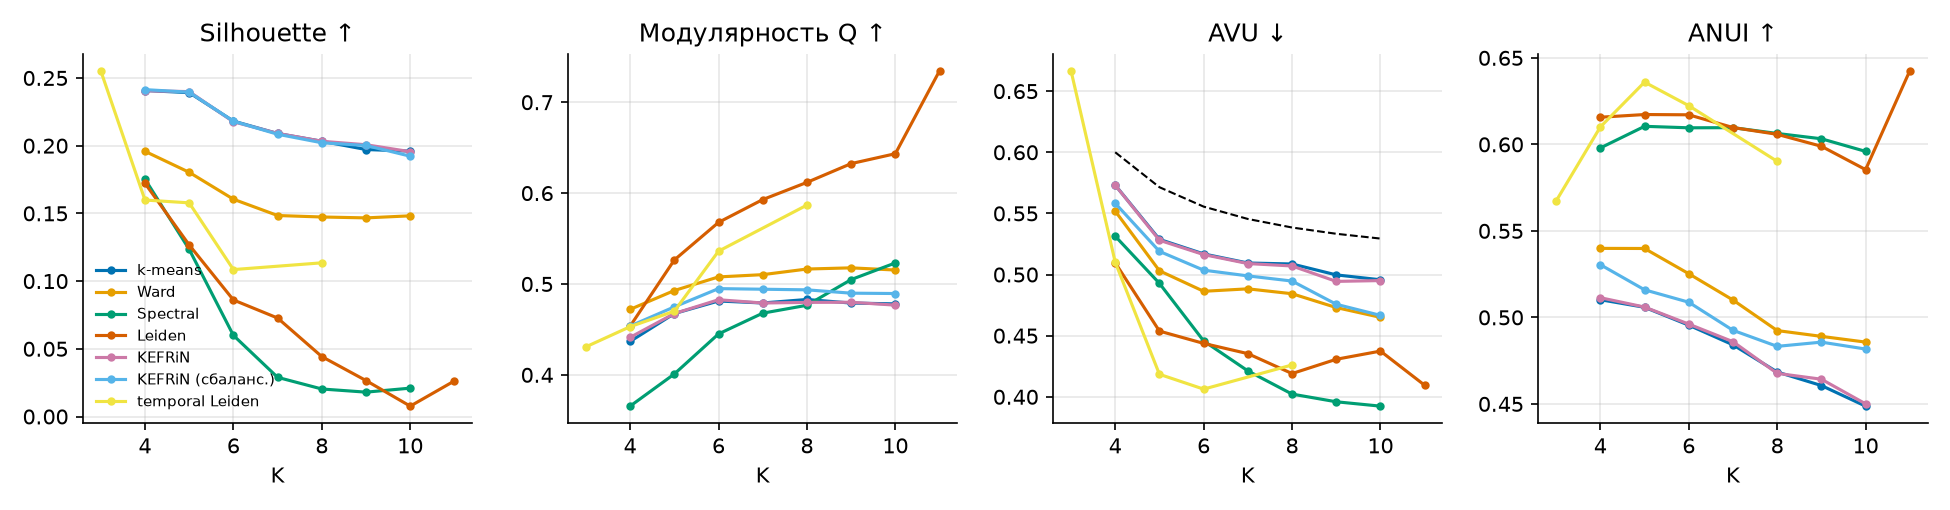
\includegraphics[width=\textwidth]{k_curves.png}
\caption{Индексы качества в зависимости от $K$; пунктир~-- уровень случайного разбиения.}
\label{fig:kcurves}
\end{figure}

\begin{figure}[htbp]
\centering
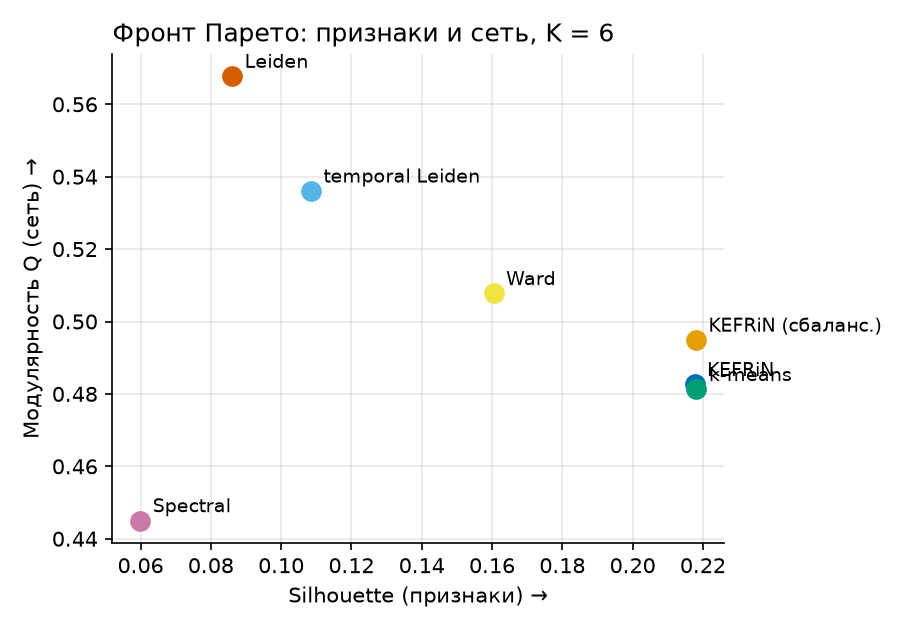
\includegraphics[width=0.62\textwidth]{pareto_sw_mq.png}
\caption{Фронт Парето <<признаки / сеть>>: SW против модулярности $Q$ при $K=6$.}
\label{fig:pareto}
\end{figure}

\begin{table}[htbp]
\centering\small
\caption{Сводные рейтинги при $K=6$. Борда по шести индексам Положения; пороговое правило Алескерова \cite{aleskerov-threshold,aleskerov-3graded}: оценки по терцилям, лексикографически по числу худших оценок; частота лидерства: доля бутстрэп-выборок месяцев, где метод лучший, усреднённая по индексам.}
\label{tab:ratings}
\begin{tabularx}{\textwidth}{>{\raggedright\arraybackslash\hspace{0pt}}p{3.2cm}>{\centering\arraybackslash\hspace{0pt}}p{1.4cm}>{\centering\arraybackslash\hspace{0pt}}X>{\centering\arraybackslash\hspace{0pt}}p{1.8cm}>{\centering\arraybackslash\hspace{0pt}}p{2.6cm}}
\toprule
Метод & Борда $\uparrow$ & Пороговое правило: оценок <<плохо / средне / хорошо>> & Ранг по порогу & Частота лидерства (бутстрэп) \\
\midrule
Leiden & 25 & 2 / 0 / 4 & 2 & 0.04 \\
temporal Leiden & 24 & 2 / 1 / 3 & 3 & 0.91 \\
Ward & 19 & 0 / 6 / 0 & 1 & 0.00 \\
KEFRiN (сбаланс.) & 16 & 3 / 2 / 1 & 4 & 0.02 \\
KEFRiN ($\rho=\xi=1$) & 15 & 4 / 1 / 1 & 7 & 0.02 \\
k-means & 14 & 4 / 0 / 2 & 6 & 0.00 \\
Spectral & 13 & 3 / 2 / 1 & 5 & 0.00 \\
\bottomrule
\end{tabularx}
\end{table}

Рейтинги расходятся (табл.~\ref{tab:ratings}). Борда и частота лидерства награждают Leiden за три сетевых индекса и S\_Dbw, пороговое правило наказывает его за провалы по SW и CH и выводит вперёд Ward; temporal Leiden набирает частоту лидерства на сетевых индексах при SW $=0{,}11$. Ни одно сводное правило не выделяет единственного победителя. Поэтому выбираем по заранее объявленным критериям: (1) Парето-эффективность, (2) отсутствие худших оценок по пороговому правилу, (3) статистически значимое преимущество над ближайшим простым методом, (4) бутстрэп-устойчивость, (5) пригодность для интерпретации (кластеры должны различаться по составу трат, иначе это не <<типы экономики>>).

\begin{table}[htbp]
\centering\footnotesize
\caption{Парный бутстрэп по 24 месяцам: разность средних и 95\,\% ДИ (ориентация <<больше~-- лучше>>). Жирным выделены ДИ, не содержащие нуля.}
\label{tab:bootstrap}

\begin{tabular}{lcccc}
\toprule
Индекс & \makecell{KEFRiN (сбаланс.)\\ $-$ k-means} & \makecell{KEFRiN (сбаланс.)\\ $-$ Ward} & \makecell{KEFRiN (сбаланс.)\\ $-$ Leiden} & \makecell{Leiden\\ $-$ k-means} \\
\midrule
SW & \makecell{$+0{,}002$\\ $[-0{,}000; +0{,}006]$} & \makecell{$\mathbf{+0{,}058}$\\ $\mathbf{[+0{,}050; +0{,}065]}$} & \makecell{$\mathbf{+0{,}128}$\\ $\mathbf{[+0{,}113; +0{,}144]}$} & \makecell{$\mathbf{-0{,}126}$\\ $\mathbf{[-0{,}139; -0{,}113]}$} \\
CH & \makecell{$\mathbf{-3}$\\ $\mathbf{[-6; -1]}$} & \makecell{$\mathbf{+119}$\\ $\mathbf{[+111; +126]}$} & \makecell{$\mathbf{+343}$\\ $\mathbf{[+327; +358]}$} & \makecell{$\mathbf{-346}$\\ $\mathbf{[-361; -331]}$} \\
S\_Dbw & \makecell{$-0{,}000$\\ $[-0{,}057; +0{,}044]$} & \makecell{$+0{,}008$\\ $[-0{,}100; +0{,}122]$} & \makecell{$\mathbf{-0{,}086}$\\ $\mathbf{[-0{,}156; -0{,}017]}$} & \makecell{$\mathbf{+0{,}085}$\\ $\mathbf{[+0{,}012; +0{,}158]}$} \\
AVI & \makecell{$\mathbf{+0{,}016}$\\ $\mathbf{[+0{,}011; +0{,}022]}$} & \makecell{$\mathbf{-0{,}016}$\\ $\mathbf{[-0{,}023; -0{,}009]}$} & \makecell{$\mathbf{-0{,}166}$\\ $\mathbf{[-0{,}174; -0{,}157]}$} & \makecell{$\mathbf{+0{,}182}$\\ $\mathbf{[+0{,}171; +0{,}193]}$} \\
AVU & \makecell{$\mathbf{+0{,}013}$\\ $\mathbf{[+0{,}009; +0{,}018]}$} & \makecell{$\mathbf{-0{,}015}$\\ $\mathbf{[-0{,}024; -0{,}006]}$} & \makecell{$\mathbf{-0{,}062}$\\ $\mathbf{[-0{,}076; -0{,}047]}$} & \makecell{$\mathbf{+0{,}075}$\\ $\mathbf{[+0{,}061; +0{,}089]}$} \\
MQ & \makecell{$\mathbf{+0{,}007}$\\ $\mathbf{[+0{,}004; +0{,}009]}$} & \makecell{$\mathbf{-0{,}018}$\\ $\mathbf{[-0{,}024; -0{,}012]}$} & \makecell{$\mathbf{-0{,}081}$\\ $\mathbf{[-0{,}096; -0{,}065]}$} & \makecell{$\mathbf{+0{,}087}$\\ $\mathbf{[+0{,}072; +0{,}102]}$} \\
ANUI & \makecell{$\mathbf{+0{,}012}$\\ $\mathbf{[+0{,}008; +0{,}017]}$} & \makecell{$\mathbf{-0{,}013}$\\ $\mathbf{[-0{,}019; -0{,}007]}$} & \makecell{$\mathbf{-0{,}109}$\\ $\mathbf{[-0{,}119; -0{,}100]}$} & \makecell{$\mathbf{+0{,}122}$\\ $\mathbf{[+0{,}111; +0{,}132]}$} \\
\bottomrule
\end{tabular}
\end{table}

Сбалансированный KEFRiN не уступает k-means ни по одному индексу признаков (разности SW и S\_Dbw незначимы) и значимо выигрывает по всем четырём сетевым (табл.~\ref{tab:bootstrap}). Против Leiden проигрыш по сети значим, но выигрыш по признакам на порядок больше по $z$. Нулевая модель графа (configuration model, фиксированные метки): $z(Q)=129$ для KEFRiN и 134 для Leiden, то есть обе типологии несут структуру сверх распределения степеней. $z(\mathrm{AVU})$ у Leiden и Spectral отрицательны ($-8$, $-20$): их разрезы <<лучше случайного>> только за счёт формы разреза, навязанной степенями.

Итог по методам. Основной метод: KEFRiN (сбалансированный). Он Парето-эффективен; по пороговому правилу уступает лишь Ward, Leiden и temporal Leiden, у которых провалы по устойчивости или по SW; значимо лучше k-means по сети при равной компактности; устойчивость ARI 0,78 при $K=6$ против 0,52 у Leiden. Из лидеров только он использует и признаки, и сеть, как требует постановка задачи. Устойчивость по бутстрэпу при $K=6$ (ARI между подвыборками, \cite{hennig}): k-means 0,81, Spectral 0,79, KEFRiN сбаланс. 0,78, Leiden 0,52, Ward 0,39. Ward, лидер порогового правила, отпадает: агломеративная иерархия перестраивается при удалении 20\,\% МО. Эффект сети мал: итоговая типология совпадает с k-means на ARI 0,91, тип отличается лишь у 4\,\% МО. Сеть сдвигает границы типов, карта в целом сохраняется; эти 4\,\% МО повышают внешнюю объяснимость зарплат с $\eta^2$ 0,47 (k-means) до 0,61 (п.~\ref{sec:external}). Leiden остаётся эталоном <<чисто сетевого>> взгляда и показан на карте как альтернативная линза.

\begin{table}[htbp]
\centering\small
\caption{Сильные стороны и ограничения методов (по табл.~\ref{tab:icvi-k6} и бутстрэп-устойчивости при $K=6$).}
\label{tab:methods-pros}
\begin{tabularx}{\textwidth}{>{\raggedright\arraybackslash\hspace{0pt}}p{2.3cm}YYY}
\toprule
Метод & Сильные стороны & Ограничения & Когда применять \\
\midrule
k-means & SW 0,218, CH 646; устойчивость ARI 0,81 & сеть не использует; MQ 0,481 & базовая линия по признакам \\
Ward & детерминирован, даёт иерархию; MQ 0,508 & устойчивость ARI 0,39; SW 0,160 & разведка структуры, не итоговая типология \\
Spectral & AVI 0,839, ANUI 0,610; устойчивость 0,79 & SW 0,060: профили не читаются & когда нужен чисто сетевой разрез \\
Leiden & MQ 0,568, AVI 0,849 & SW 0,086; устойчивость 0,52 & эталон сетевых сообществ, альтернативная линза \\
temporal Leiden & сквозные метки по построению (ARI соседних месяцев 0,95); ANUI 0,622 & несбалансирован: при $K=4$ крупнейшее сообщество 71\,\% МО; SW 0,108 & когда важна непрерывность меток, а не баланс типов \\
KEFRiN ($\rho=\xi=1$) & учитывает и признаки, и сеть; SW 0,218 & сеть почти не влияет: ARI с k-means 0,97 & при сопоставимых масштабах признаков и сети \\
KEFRiN (сбаланс.) & SW 0,218 при MQ 0,495 и ANUI 0,509; устойчивость 0,78 & сетевые индексы ниже, чем у Leiden & основной метод: признаки и сеть вместе \\
\bottomrule
\end{tabularx}
\end{table}


\begin{table}[htbp]
\centering\small
\caption{Выбор $K$ для KEFRiN (сбаланс.). Три критерия, объявленных заранее: $z_{\mathrm{AVU}}$ (единственный сетевой индекс с пиком по $K$), $z_{\mathrm{SW}}$ и бутстрэп-устойчивость (10 подвыборок по 80\,\% МО, медиана ARI между подвыборками).}
\label{tab:k-select}
\begin{tabular}{crrrrcc}
\toprule
$K$ & $z_{\mathrm{SW}}$ & $z_{\mathrm{AVU}}$ & $z_{\mathrm{MQ}}$ & SW & \makecell{устойчивость\\ ARI (бутстрэп)} & \makecell{Жаккар худшего\\ кластера} \\
\midrule
4 & 40{,}4 & 6{,}5 & 97 & 0{,}241 & 0{,}89 & 0{,}76 \\
5 & 30{,}5 & 9{,}1 & 106 & 0{,}240 & 0{,}86 & 0{,}86 \\
6 & 26{,}2 & 16{,}5 & 114 & 0{,}218 & 0{,}78 & 0{,}78 \\
7 & 20{,}7 & 2{,}7 & 116 & 0{,}208 & 0{,}67 & 0{,}46 \\
8 & 24{,}9 & 4{,}4 & 124 & 0{,}202 & 0{,}61 & 0{,}51 \\
9 & 14{,}9 & 0{,}2 & 132 & 0{,}200 & 0{,}53 & 0{,}46 \\
10 & 13{,}5 & $-5{,}9$ & 140 & 0{,}192 & 0{,}56 & 0{,}37 \\
\bottomrule
\end{tabular}
\end{table}

Двухшаговое правило (табл.~\ref{tab:k-select}). \textit{Шаг~1}: сумма нормированных критериев выбирает $K=4$ (укрупнённые группы: города и столичные районы; малые города и сельская периферия; часть северных территорий; смешанная группа районов на трассах). Ближайший кандидат $K=6$ имеет максимальный $z_{\mathrm{AVU}}$, вложен в $K=4$ на 82\,\% (доля МО, чей подтип целиком лежит в одном макротипе) и добавляет два содержательных и устойчивых типа: мегаполисы отделяются от крупных городов, Север отделяется от промышленных городов. \textit{Шаг~2}: среди $K>4$ выбирается ближайший уровень, где $z_{\mathrm{AVU}}$ максимален, а худший по Жаккару кластер устойчив ($\ge 0{,}75$); это $K=6$. Основной уровень типологии составляют 6 подтипов, макроуровень $K=4$ служит агрегацией; оба уровня воспроизводятся из одних файлов (\code{outputs/compare/k_selection.csv}). Ограничение: метод, $K$ и балансировка выбирались по всем 24 месяцам, включая 2024~г.; без будущего строятся только признаки, граф и онлайн-разметка п.~\ref{sec:oot}.

Temporal Leiden ($\omega=0{,}25$, сетка $K\in\{4,6,8\}$) даёт сквозные метки по построению (ARI соседних месяцев 0,95), но разбиение сильно несбалансировано (при $K=4$ крупнейшее сообщество охватывает 71\,\% МО), при $K=6$ SW $=0{,}11$, $Q=0{,}54$ (табл.~\ref{tab:icvi-k6}). При $\omega=0{,}5$ бисекция по $\gamma$ давала вырожденное решение (одно сообщество на 90\,\% узлов). Как единая модель динамики он проигрывает связке <<помесячный KEFRiN + подтверждённые переходы>> и по качеству, и по читаемости; подробности в прил.~\ref{app:ablation}.

%=====================================================================
\section{Типы локальных экономик}\label{sec:types}

\subsection{Паспорта типов}\label{sec:passports}

Тип МО определяется как модальный подтверждённый тип за 2024~г. (у 84,9\,\% МО он совпадает с типом в опорном месяце 2023-12). Профили по Миркину \cite{mirkin-book} объясняют $B/T=62{,}8$\,\% дисперсии признаков. Дерево решений глубины 3 на исходных единицах (доли в \%, траты в рублях) воспроизводит типы с точностью 77\,\% (кросс-валидация 74\,\%), то есть каждый тип описывается тремя-четырьмя порогами, понятными без модели (рис.~\ref{fig:tree}).

\begin{table}[htbp]
\centering\footnotesize
\caption{Паспорта типов: медианы по МО типа (2024~г.). Доли~-- в \% от итога трат; зарплата и население взяты из Росстата и в кластеризации не участвовали.}
\label{tab:passports}
\setlength{\tabcolsep}{2.4pt}
\begin{tabularx}{\textwidth}{>{\raggedright\arraybackslash\hspace{0pt}}X>{\centering\arraybackslash\hspace{0pt}}p{1.55cm}>{\centering\arraybackslash\hspace{0pt}}p{1.9cm}*{6}{>{\centering\arraybackslash\hspace{0pt}}p{1.06cm}}>{\centering\arraybackslash\hspace{0pt}}p{1.15cm}>{\centering\arraybackslash\hspace{0pt}}p{1.05cm}}
\toprule
Тип & МО & \makecell{Траты на\\ жителя, \rub\\ (\% к мед.)} & Продо\-воль\-ствие & Здо\-ровье & Марке\-т\-плей\-сы & Обще\-пит & Транс\-порт & Прочее & \makecell{Зарпла-\\та, \rub} & \makecell{Насе-\\ление,\\ тыс.} \\
\midrule
Сельская периферия & 424 (21\,\%) & 21\,868 (82\,\%) & 47,8 & 5,0 & 19,2 & 1,2 & 5,1 & 21,3 & 40\,183 & 13 \\
Промышленные города и пригороды & 399 (20\,\%) & 32\,336 (121\,\%) & 40,4 & 4,8 & 15,2 & 4,4 & 6,2 & 29,0 & 58\,310 & 61 \\
Малые города и райцентры & 440 (22\,\%) & 24\,614 (92\,\%) & 45,8 & 4,4 & 17,2 & 2,0 & 4,2 & 25,7 & 47\,426 & 20 \\
Аграрные районы на трассах & 319 (16\,\%) & 23\,795 (89\,\%) & 46,1 & 4,5 & 15,1 & 2,0 & 6,0 & 26,0 & 46\,035 & 19 \\
Мегаполисы и столичные районы & 318 (16\,\%) & 49\,560 (186\,\%) & 32,4 & 5,6 & 13,0 & 7,6 & 7,2 & 33,9 & 108\,118 & 84 \\
Север и ресурсные территории & 116 (6\,\%) & 41\,098 (154\,\%) & 42,7 & 3,6 & 10,1 & 3,7 & 4,7 & 33,3 & 104\,926 & 18 \\
\midrule
\multicolumn{11}{l}{\textit{Типичные МО}} \\
\multicolumn{11}{>{\raggedright\arraybackslash}p{\dimexpr\linewidth-2\tabcolsep}}{Сельская периферия: Хотынецкий, Мучкапский, Барышский} \\
\multicolumn{11}{>{\raggedright\arraybackslash}p{\dimexpr\linewidth-2\tabcolsep}}{Промышленные города и пригороды: Беловский, Сызрань, Сысертский} \\
\multicolumn{11}{>{\raggedright\arraybackslash}p{\dimexpr\linewidth-2\tabcolsep}}{Малые города и райцентры: Козьмодемьянск, Дегтярск, Еткульский} \\
\multicolumn{11}{>{\raggedright\arraybackslash}p{\dimexpr\linewidth-2\tabcolsep}}{Аграрные районы на трассах: Чистоозерный, Тогучинский, Карагайский} \\
\multicolumn{11}{>{\raggedright\arraybackslash}p{\dimexpr\linewidth-2\tabcolsep}}{Мегаполисы и столичные районы: Чертаново Центральное, Орехово-Борисово Северное, Ясенево} \\
\multicolumn{11}{>{\raggedright\arraybackslash}p{\dimexpr\linewidth-2\tabcolsep}}{Север и ресурсные территории: Охинский, Зейский, Заполярный} \\
\bottomrule
\end{tabularx}
\end{table}

\paragraph{Сельская периферия.} Самый низкий уровень трат (82\,\% медианы страны). Почти половина уходит на продовольствие, общепита практически нет, аптеки и маркетплейсы заметны как замена офлайн-торговли. Муниципальные районы Черноземья, Поволжья и юга Сибири с сельским населением, низкими зарплатами (около 40~тыс.~\rub) и занятостью в образовании и сельском хозяйстве.

\paragraph{Промышленные города и пригороды.} Траты выше среднего (121\,\% медианы), доля продовольствия ниже, общепит заметен. Города и городские округа с преобладанием городского населения, зарплатой около 58~тыс.~\rub{} и обрабатывающей промышленностью как главной отраслью: индустриальный Урал, Кузбасс, Подмосковье, Поволжье.

\paragraph{Малые города и райцентры.} Уровень трат чуть ниже среднего (92\,\%), структура смешанная: продовольствие и маркетплейсы выше среднего, транспорт ниже. Малые города и районы с райцентром в Центре, Поволжье и на Урале, зарплата около 47~тыс.~\rub{} Самый <<переходный>> тип: граничит и с селом, и с промышленными городами.

\paragraph{Аграрные районы на трассах.} Низкий уровень трат (89\,\%) при повышенной доле транспорта (топливо, переезды). Чисто сельские районы вдоль магистралей и в республиках Поволжья, Алтая и Забайкалья, с худшей доступностью рынков среди <<материковых>> типов. Самый подвижный тип: чаще других меняет принадлежность.

\paragraph{Мегаполисы и столичные районы.} Траты почти вдвое выше медианы страны (186\,\%), на продовольствие приходится лишь треть, доли общепита и транспорта максимальные. Внутригородские территории Москвы и Петербурга (233 из 318 МО типа) и крупнейшие региональные центры; зарплата свыше 100~тыс.~\rub, максимальная доступность рынков. Самый устойчивый тип.

\paragraph{Север и ресурсные территории.} Высокий уровень трат (154\,\%) при большой доле <<прочих>> категорий и вдвое меньшей доле маркетплейсов: логистика дорогая, онлайн-канал слабый. Якутия, ЯНАО, Сахалин, север Красноярского края и Коми; зарплата свыше 100~тыс.~\rub, доля добывающих отраслей втрое выше медианы, доступность рынков минимальная.

\medskip
Рис.~\ref{fig:profiles} показывает профили в $\sigma$; полные паспорта с типичными и пограничными МО есть на лендинге и в \code{outputs/interpret/types_summary.json}.

\begin{figure}[htbp]
\centering
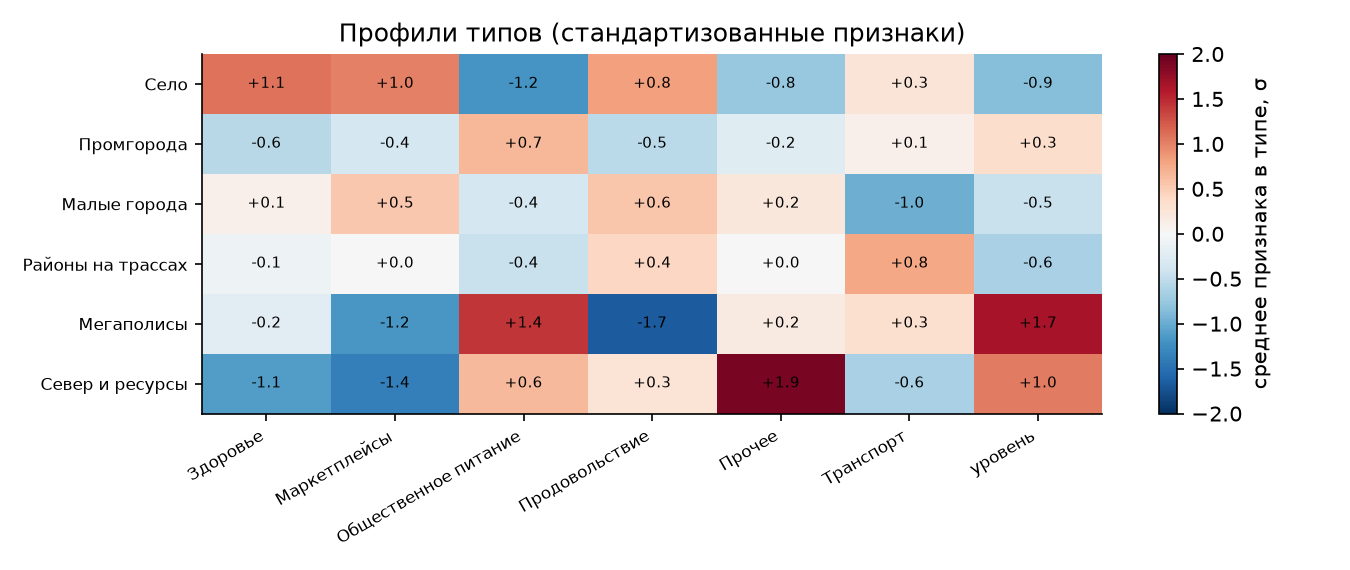
\includegraphics[width=\textwidth]{profiles.png}
\caption{Профили типов в единицах стандартного отклонения признаков.}
\label{fig:profiles}
\end{figure}

\begin{figure}[htbp]
\centering
\small
\begin{minipage}{0.9\textwidth}
\begin{itemize}[label={},leftmargin=0pt,itemsep=1pt]
\item Доля <<Общественное питание>> $\le 3{,}3$\,\%
  \begin{itemize}[label={},leftmargin=1.2em,itemsep=1pt,topsep=1pt]
  \item Доля <<Транспорт>> $\le 4{,}8$\,\%
    \begin{itemize}[label={},leftmargin=1.2em,itemsep=1pt,topsep=1pt]
    \item Доля <<Прочее>> $\le 21{,}8$\,\% $\Rightarrow$ \textbf{Село}
    \item Доля <<Прочее>> $> 21{,}8$\,\% $\Rightarrow$ \textbf{Малые города}
    \end{itemize}
  \item Доля <<Транспорт>> $> 4{,}8$\,\%
    \begin{itemize}[label={},leftmargin=1.2em,itemsep=1pt,topsep=1pt]
    \item Доля <<Прочее>> $\le 23{,}3$\,\% $\Rightarrow$ \textbf{Село}
    \item Доля <<Прочее>> $> 23{,}3$\,\% $\Rightarrow$ \textbf{Районы на трассах}
    \end{itemize}
  \end{itemize}
\item Доля <<Общественное питание>> $> 3{,}3$\,\%
  \begin{itemize}[label={},leftmargin=1.2em,itemsep=1pt,topsep=1pt]
  \item Доля <<Общественное питание>> $\le 5{,}9$\,\%
    \begin{itemize}[label={},leftmargin=1.2em,itemsep=1pt,topsep=1pt]
    \item Доля <<Прочее>> $\le 32{,}6$\,\% $\Rightarrow$ \textbf{Промгорода}
    \item Доля <<Прочее>> $> 32{,}6$\,\% $\Rightarrow$ \textbf{Север и ресурсы}
    \end{itemize}
  \item Доля <<Общественное питание>> $> 5{,}9$\,\%
    \begin{itemize}[label={},leftmargin=1.2em,itemsep=1pt,topsep=1pt]
    \item Итог на жителя $\le 36\,654{,}1$ \rub{} $\Rightarrow$ \textbf{Промгорода}
    \item Итог на жителя $> 36\,654{,}1$ \rub{} $\Rightarrow$ \textbf{Мегаполисы}
    \end{itemize}
  \end{itemize}
\end{itemize}
\end{minipage}
\caption{Правила дерева решений глубины 3 (сокращённо; полностью в \texttt{rule\_tree.txt}, каталог \texttt{outputs/interpret}).}
\label{fig:tree}
\end{figure}

\subsection{Внешняя проверка на данных, не входивших в кластеризацию}\label{sec:external}

\begin{table}[htbp]
\centering\small
\caption{Связь типов с внешними переменными. $\eta^2_H$~-- доля дисперсии, объяснённая типом, по Краскелу--Уоллису; $V$ Крамера для категориальных; все переменные вне признаков кластеризации.}
\label{tab:external}
\begin{tabularx}{\textwidth}{Ylcc}
\toprule
Внешняя переменная & Статистика & Сила связи & $p$ \\
\midrule
Регион (справочник) & $V$ Крамера & 0.63 & $<0{,}001$ \\
Средняя зарплата (Росстат) & $\eta^2_H$ & 0.61 & $<0{,}001$ \\
Тип МО (район / округ / внутригородская территория) & $V$ Крамера & 0.54 & $<0{,}001$ \\
Число работников организаций & $\eta^2_H$ & 0.50 & $<0{,}001$ \\
Население & $\eta^2_H$ & 0.48 & $<0{,}001$ \\
Доля городского населения & $\eta^2_H$ & 0.47 & $<0{,}001$ \\
Индекс доступности рынков (СберИндекс) & $\eta^2_H$ & 0.35 & $<0{,}001$ \\
Ведущая отрасль занятости & $V$ Крамера & 0.35 & $<0{,}001$ \\
Доля бюджетного сектора в занятости & $\eta^2_H$ & 0.23 & $<0{,}001$ \\
Статус (центр субъекта / ЗАТО) & $V$ Крамера & 0.22 & $<0{,}001$ \\
Работников на жителя & $\eta^2_H$ & 0.16 & $<0{,}001$ \\
Доля добычи и энергетики в занятости & $\eta^2_H$ & 0.16 & $<0{,}001$ \\
Концентрация занятости (HHI) & $\eta^2_H$ & 0.03 & $<0{,}001$ \\
\bottomrule
\end{tabularx}
\end{table}

Базовые линии. Чтобы $\eta^2=0{,}61$ по зарплате что-то значило, его нужно сравнить с простыми альтернативами. Шесть групп МО только по уровню трат объясняют зарплату лучше ($\eta^2$ 0,72), регион даёт 0,70, k-means на тех же признаках 0,47, административный тип МО 0,36; без внутригородских территорий Москвы и Петербурга типы дают 0,48, уровень трат 0,62. Значит, по зарплате типология уступает одномерной шкале <<богатства>>: типы различают ещё и структуру трат (село с маркетплейсами против села с продовольствием при одинаковом уровне). При этом по зарплате она информативнее k-means на тех же признаках (0,61 против 0,47) за счёт сети и балансировки. Поэтому ниже акцент сделан на переменных структуры экономики (отрасли, урбанизация, доступность рынков).

Что сходится (табл.~\ref{tab:external}): типы объясняют 61\,\% разброса зарплат и 48\,\% разброса населения, хотя ни того ни другого модель не видела; административный тип МО связан с типологией с $V=0{,}54$; доступность рынков минимальна у Севера и максимальна у мегаполисов; у Севера доля добывающих отраслей втрое выше медианы. Что не сходится и почему. Регион объясняет типологию сильнее всего ($V=0{,}63$): отчасти это география экономики, отчасти региональные особенности безналичного охвата. Ведущая отрасль занятости по Росстату (без малого бизнеса) связана с типами слабее зарплаты ($V=0{,}35$): у малых МО это почти всегда <<образование>>, а торговля и услуги, формирующие траты, в выборке Росстата недопредставлены.

%=====================================================================
\section{Динамика}\label{sec:dynamics}

\subsection{Сквозные типы и подтверждённые переходы}\label{sec:transitions}

Метки месяцев связываются венгерским сопоставлением по Жаккару; номера типов присваиваются по убыванию размера в опорном месяце 2023-12. Сырые помесячные метки подвержены частым сменам типа: 4\,112 смен типа за 23 перехода, без единой смены остаются лишь 36,7\,\% МО. Правило подтверждения (новый тип держится не менее 3 месяцев подряд, и средняя бутстрэп-вероятность назначенного типа за эти месяцы не ниже 0,7) оставляет 963 подтверждённые смены у 651 МО; 67,7\,\% МО не меняют тип ни разу. Разложение сырых смен: 67,9\,\% составляет шум (новый тип продержался меньше трёх месяцев или МО вернулось в прежний тип), 23,4\,\% подтверждены, остальное приходится на <<кандидатов>> в хвосте ряда (ещё не прошло три месяца). Сезонность видна и после фильтра: подтверждённые смены чаще начинаются в июне и январе (в 2,2 и 2,1 раза чаще равномерного), 4,4\,\% смен приходятся на пару декабрь$\to$январь, 3,9\,\% повторяются у того же МО ровно через 12 месяцев.

Индекс Шоррокса \cite{shorrocks} матрицы переходов $P$:
\begin{equation}\label{eq:shorrocks}
M=\frac{K-\mathrm{tr}\,P}{K-1}.
\end{equation}
По сырым меткам $M$ равен 0,155 (lag 1) и 0,413 (lag 12), по подтверждённым 0,023 и 0,208. Здесь lag~1 и lag~12 – среднее по всем парам месяцев, отстоящих на 1 и 12 месяцев; одна годовая пара декабрь 2023 $\to$ декабрь 2024 даёт 0,169 (в аннотации округлено до 0,17). Диагональ годовой матрицы (рис.~\ref{fig:dynamics}): мегаполисы 0,96, Север 0,90, промышленные города 0,88, село 0,85, малые города 0,82, аграрные районы на трассах 0,75. Последний тип самый подвижный, и его главный обмен идёт с малыми городами (50 МО туда, 32 обратно). События жизненного цикла \cite{greene,rossetti} по Greene \cite{greene} (порог Жаккара 0,3) на подтверждённых типах сводятся к \texttt{continue} (138 событий): за два года ни один тип не родился, не умер, не слился и не разделился. Меняются отдельные МО, сами типы сохраняются.

\begin{figure}[htbp]
\centering
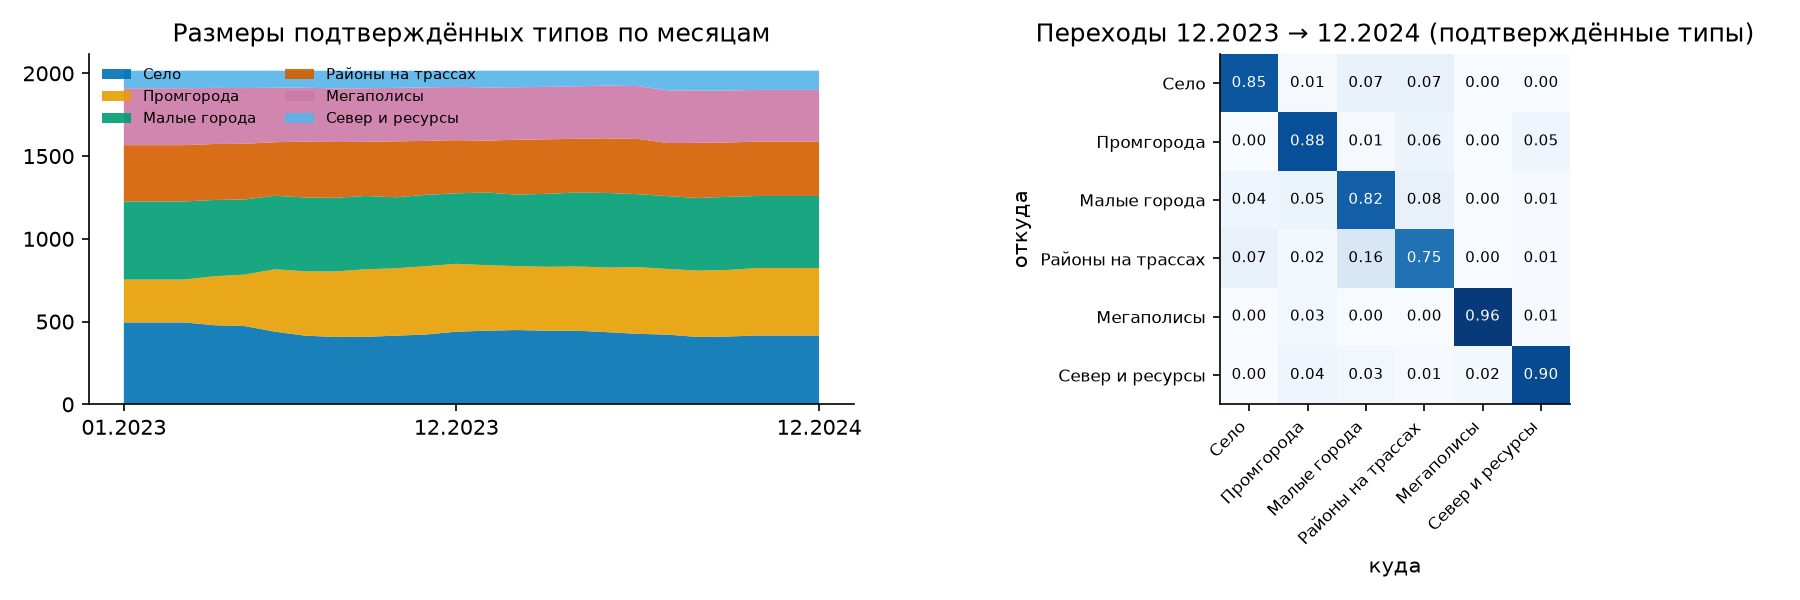
\includegraphics[width=\textwidth]{dynamics.png}
\caption{Размеры подтверждённых типов по месяцам и матрица переходов через 12 месяцев.}
\label{fig:dynamics}
\end{figure}

Бутстрэп-уверенность (30 подвыборок по 80\,\% МО, выравнивание к опорному разбиению): медиана 0,97, у 90\,\% пар <<МО $\times$ месяц>> уверенность $\ge 0{,}7$; на карте она показана прозрачностью. Оговорки: подтверждение ретроспективно на два месяца (месяц, когда смена становится известна онлайн, хранится отдельно в \code{confirmed_month}); подвыборки по 80\,\% мало сдвигают центры, поэтому уверенность скорее завышена.

\subsection{Out-of-time: 2023 \texorpdfstring{$\to$}{→} 2024}\label{sec:oot}

Проверка динамики идёт без данных будущего: центры типов считаются только по 12 месяцам 2023~г., каждый месяц 2024~г. классифицируется ближайшим центром без пересчёта. Согласие онлайн-разметки с полной (где 2024~г. участвовал в кластеризации): ARI 0,68, совпадение типа у 84,2\,\% МО. Согласие падает с 0,78 в январе до 0,65 в декабре, потому что центры типов дрейфуют, прежде всего из-за волны маркетплейсов (п.~\ref{sec:cases}). Из 682 подтверждённых смен 2024~г. онлайн-режим воспроизводит 265 (полнота 0,39, точность 0,47; с точным месяцем 0,16): часть <<смен>> полной разметки отражает движение центров типов при неизменных МО. Годовой Шоррокс онлайн равен 0,238 против 0,169 в полной разметке.

\subsection{Кейсы}\label{sec:cases}

\paragraph{Орск: паводок апреля 2024.} 5 апреля 2024~г. прорыв дамбы в Орске затопил часть города. В данных СберИндекса уровень трат почти не изменился (отношение к медиане страны держится на 1,15--1,25 весь 2024 год), сдвинулась структура: доля продовольствия подскакивает с 37,9\,\% до 40,1\,\%, доля маркетплейсов падает с 14,0\,\% до 12,4\,\% (логистика), здоровья с 4,7\,\% до 4,2\,\%. Тип МО (<<промышленные города и пригороды>>) не меняется, но бутстрэп-уверенность в нём падает с 0,83--1,00 до 0,50--0,57 в июне--сентябре 2024~г. и восстанавливается к декабрю; на карте это видно как более бледная заливка МО в режиме <<слой неопределённости>>.

\paragraph{Апрель 2023: методологический разрыв.} В апреле 2023~г. у 30--38\,\% МО синхронно падают оценки по <<Здоровью>> (медианно $-17$\,\%) и <<Общепиту>> ($-18$\,\%) при почти неизменном итоге. Это признак смены методики оценки; с поведением жителей разрыв не связан. Помесячная кластеризация реагирует: 567 сырых смен типа в апреле против 90--230 в соседних месяцах. Правило подтверждения (новый тип $\ge 3$ месяцев и бутстрэп-уверенность $\ge 0{,}7$) оставляет из них 62. Подсчёт смен типа по сырым меткам показал бы в этом месяце массовую перестройку, которой в экономике не было.

\paragraph{Объединения МО 2024 года: Павлово-Посадский и Сасовский округа.} С марта 2024~г. Павловский Посад и Электрогорск объединены в Павлово-Посадский округ (\code{union_22}), Сасово и Сасовский район объединены в Сасовский округ (\code{union_23}). В данных предшественники живут по февраль 2024~г., преемники появляются с марта, поэтому ни те ни другие не входят в обучающую панель полной истории и классифицируются по ближайшему центру типа в каждом месяце. На них проверяется устойчивость типологии к новым объектам. Павлово-Посадский округ наследует тип обоих предшественников (промышленные города и пригороды, все 10 месяцев); Сасовский округ наследует тип города Сасово (малые города) в 8 из 10 месяцев, потому что город доминирует в тратах объединённой территории. Смена идентификатора МО ложной смены типа не создаёт.

\paragraph{Волна маркетплейсов: село догоняет, Север отстаёт.} За два года медианная доля маркетплейсов в тратах удвоилась во всех типах: в сельской периферии с 11,4\,\% до 22,8\,\%, в промышленных городах с 9,3\,\% до 18,4\,\%, в мегаполисах с 8,5\,\% до 16,0\,\% (рис.~\ref{fig:marketplaces}). Онлайн-канал растёт быстрее всего там, где офлайн-торговли меньше, отсюда <<догоняющее село>>. Север и ресурсные территории растут в разах не медленнее (5,1\,\% $\to$ 12,5\,\%), но их доля весь период остаётся вдвое ниже остальных: разрыв в онлайн-доступе сохраняется из-за логистики. Признаки центрируются внутри месяца, поэтому эта общестрановая волна не создаёт ложных смен типа (в отличие от решений, где доли берутся как есть). Она видна как сдвиг центров типов, из-за которого онлайн-классификация 2024 года по центрам 2023-го даёт ARI 0,68.

\begin{figure}[htbp]
\centering
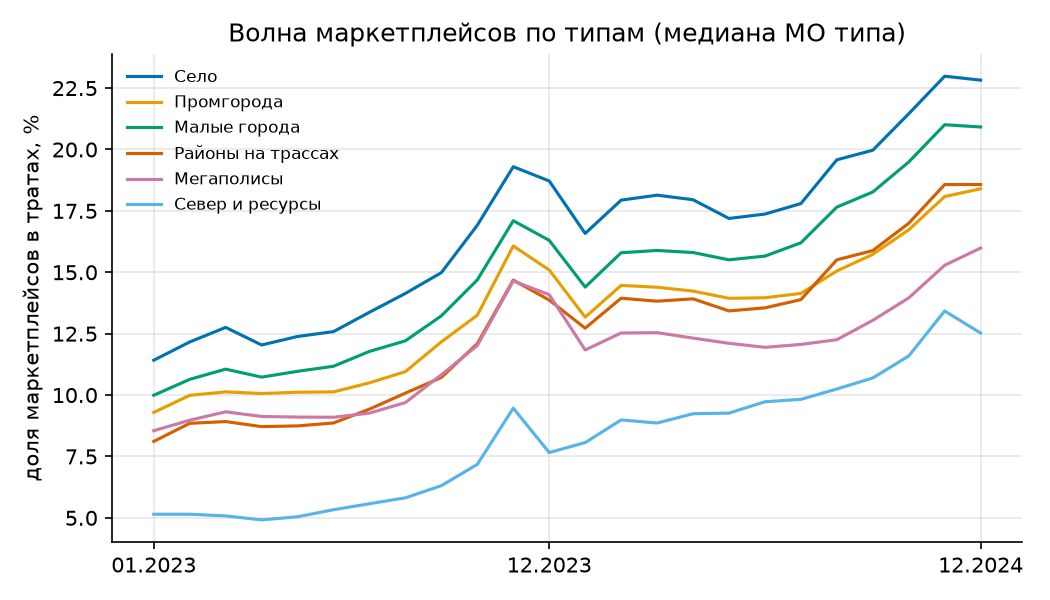
\includegraphics[width=0.75\textwidth]{marketplaces.png}
\caption{Медианная доля маркетплейсов в тратах по типам, 2023--2024~гг.}
\label{fig:marketplaces}
\end{figure}

Каждый кейс воспроизводится из артефактов \code{outputs/} (источники перечислены в \code{docs/cases.json}) и показан на лендинге кнопкой <<показать на карте>>.

%=====================================================================
\section{Выводы, ограничения, дальнейшая работа}\label{sec:conclusions}

\subsection*{Выводы}
\begin{enumerate}
\item В безналичных тратах устойчиво читаются шесть типов локальных экономик, и они совпадают с экономической географией страны, проверенной независимыми данными.
\item Правило ребра меняет сеть сильнее, чем типологию: слои почти не пересекаются (Жаккар рёбер 0,02--0,04), но при разумном весе признаков итоговые типы устойчивы к слою; сеть уточняет границы типов (прил.~\ref{app:ablation}).
\item Сравнение методов без доверительных интервалов вводит в заблуждение: разные сводные правила дают разных лидеров, и выбрать метод обоснованно можно только по явным критериям (Парето-эффективность, отсутствие провалов, значимость, устойчивость, читаемость).
\item Большая часть <<динамики>> помесячной кластеризации оказывается шумом: из 4\,112 сырых смен подтверждаются 963, а онлайн-проверка показывает, что и среди них часть объясняется дрейфом центров.
\item Для практики карта с уверенностью полезнее самих меток: шок виден по падению уверенности при неизменном типе.
\end{enumerate}

\subsection*{Кому и зачем}
Региональным органам и аналитикам типология даёт четыре инструмента. (1) Перечень МО с подтверждённой сменой типа – сигнал для проверки. (2) Падение бутстрэп-уверенности ниже 0,7 – индикатор шока без смены типа: у Орска она опускалась до 0,50–0,57 в июне–сентябре 2024~г. при обычных 0,83–1,00. (3) Подбор сопоставимых МО по типу для сравнения политик. (4) Разрыв в онлайн-доступе Севера: доля маркетплейсов 12,5\,\% против 16–23\,\% у остальных типов в декабре 2024~г. В 2024~г. у 296 МО (14,7\,\%) подтверждённый тип в декабре отличается от декабря 2023~г.; список с месяцем подтверждения (\code{confirmed_month}) выгружается из \code{outputs/dynamics} и может служить ежемесячным реестром для проверки. Уровень трат лучше предсказывает зарплату ($\eta^2$ 0,72), но только типология отличает Север от мегаполисов при близком уровне трат (154\,\% против 186\,\% медианы) и даёт структуру трат.

\subsection*{Ограничения}
Панель включает только МО с оценками, прошедшими порог качества (нет 8 регионов и части малых МО); траты безналичные и только клиентов Сбера, что смещает уровень в пользу городов; апрельский разрыв 2023~г. вызван сменой методики; внутригородские территории Москвы и Петербурга не являются самостоятельными экономиками и образуют отдельный тип из-за устройства данных; подтверждение перехода ретроспективно на 2 месяца (месяц, когда смена становится известна онлайн, хранится отдельно).

\subsection*{Дальнейшая работа}
Трикластеризация \cite{ignatov2015,ganter} куба МО $\times$ категория $\times$ месяц; совместная модель <<типология + переходы>> (скрытая марковская модель на центрах типов) вместо правила подтверждения; добавление категорий трат при расширении набора; проверка типов на данных индекса мобильности по всем регионам, когда они появятся.

%=====================================================================
\begin{thebibliography}{99}
\small
\bibitem{shalileh-eswa} Shalileh S., Antonov E., Tsyplakova D. Internal cluster validity indices for attributed networks: A controlled comparative study // Expert Systems with Applications. 2026. Vol.~333. Art.~133912. DOI: 10.1016/j.eswa.2026.133912.
\bibitem{shalileh-doklady} Shalileh S., Antonov E.\,A., Tsyplakova D.\,A. Cluster Validity across Attribute and Network Spaces: Empirical Benchmarks for Attributed Networks Clustering // Doklady Mathematics. 2025. Vol.~112, No.~3. P.~553--564. DOI: 10.1134/S1064562425700589.
\bibitem{shalileh-profiling} Shalileh S., Antonov E., Tsyplakova D. Profiling Consumption Using Attributed Network Clustering // Complex Networks \& Their Applications XIV. Studies in Computational Intelligence. Cham: Springer, 2026. P.~77--88. DOI: 10.1007/978-3-032-16723-1\_7.
\bibitem{shalileh-mirkin-entropy} Shalileh S., Mirkin B. Community Partitioning over Feature-Rich Networks Using an Extended K-Means Method // Entropy. 2022. Vol.~24, No.~5. Art.~626. DOI: 10.3390/e24050626.
\bibitem{biswas} Biswas A., Biswas B. Defining quality metrics for graph clustering evaluation // Expert Systems with Applications. 2017. Vol.~71. P.~1--17. DOI: 10.1016/j.eswa.2016.11.011.
\bibitem{howie} Howie J., Srinivasan V., Thomo A. Scaling Up Structural Clustering to Large Probabilistic Graphs Using Lyapunov Central Limit Theorem // Proc. VLDB Endowment. 2023. Vol.~16, No.~11. P.~3165--3177. DOI: 10.14778/3611479.3611516.
\bibitem{rousseeuw} Rousseeuw P.\,J. Silhouettes: a graphical aid to the interpretation and validation of cluster analysis // J. Comput. Appl. Math. 1987. Vol.~20. P.~53--65. DOI: 10.1016/0377-0427(87)90125-7.
\bibitem{calinski} Caliński T., Harabasz J. A dendrite method for cluster analysis // Communications in Statistics. 1974. Vol.~3, No.~1. P.~1--27. DOI: 10.1080/03610927408827101.
\bibitem{davies} Davies D.\,L., Bouldin D.\,W. A Cluster Separation Measure // IEEE TPAMI. 1979. Vol.~PAMI-1, No.~2. P.~224--227. DOI: 10.1109/TPAMI.1979.4766909.
\bibitem{halkidi} Halkidi M., Vazirgiannis M. Clustering validity assessment: finding the optimal partitioning of a data set // Proc. IEEE ICDM 2001. P.~187--194. DOI: 10.1109/ICDM.2001.989517.
\bibitem{newman} Newman M.\,E.\,J., Girvan M. Finding and evaluating community structure in networks // Physical Review E. 2004. Vol.~69. 026113. DOI: 10.1103/PhysRevE.69.026113.
\bibitem{mancoridis} Mancoridis S., Mitchell B.\,S., Rorres C., Chen Y., Gansner E.\,R. Using automatic clustering to produce high-level system organizations of source code // Proc. IWPC'98. IEEE, 1998. P.~45--52. DOI: 10.1109/WPC.1998.693283.
\bibitem{mitchell} Mitchell B.\,S., Mancoridis S. On the automatic modularization of software systems using the Bunch tool // IEEE Trans. Software Engineering. 2006. Vol.~32, No.~3. P.~193--208. DOI: 10.1109/TSE.2006.31.
\bibitem{mirkin-book} Mirkin B. Clustering: A Data Recovery Approach. 2nd ed. Boca Raton: CRC Press, 2012.
\bibitem{mirkin-core} Mirkin B. Core Concepts in Data Analysis: Summarization, Correlation and Visualization. London: Springer, 2011.
\bibitem{aleskerov-threshold} Aleskerov F., Chistyakov V.\,V., Kalyagin V. The threshold aggregation // Economics Letters. 2010. Vol.~107, No.~2. P.~261--262. DOI: 10.1016/j.econlet.2010.01.041.
\bibitem{aleskerov-3graded} Aleskerov F.\,T., Yakuba V.\,I., Yuzbashev D.\,A. A `threshold aggregation' of three-graded rankings // Mathematical Social Sciences. 2007. Vol.~53. P.~106--110.
\bibitem{ignatov2015} Ignatov D.\,I., Gnatyshak D.\,V., Kuznetsov S.\,O., Mirkin B.\,G. Triadic Formal Concept Analysis and triclustering: searching for optimal patterns // Machine Learning. 2015. Vol.~101, No.~1--3. P.~271--302. DOI: 10.1007/s10994-015-5487-y.
\bibitem{ganter} Ganter B., Wille R. Formal Concept Analysis: Mathematical Foundations. Berlin: Springer, 1999.
\bibitem{mucha} Mucha P.\,J., Richardson T., Macon K., Porter M.\,A., Onnela J.-P. Community Structure in Time-Dependent, Multiscale, and Multiplex Networks // Science. 2010. Vol.~328, No.~5980. P.~876--878. DOI: 10.1126/science.1184819.
\bibitem{greene} Greene D., Doyle D., Cunningham P. Tracking the Evolution of Communities in Dynamic Social Networks // Proc. ASONAM 2010. IEEE. P.~176--183. DOI: 10.1109/ASONAM.2010.17.
\bibitem{rossetti} Rossetti G., Cazabet R. Community Discovery in Dynamic Networks: A Survey // ACM Computing Surveys. 2018. Vol.~51, No.~2. Art.~35. DOI: 10.1145/3172867.
\bibitem{shorrocks} Shorrocks A.\,F. The Measurement of Mobility // Econometrica. 1978. Vol.~46, No.~5. P.~1013--1024. DOI: 10.2307/1911433.
\bibitem{traag} Traag V.\,A., Waltman L., van Eck N.\,J. From Louvain to Leiden: guaranteeing well-connected communities // Scientific Reports. 2019. Vol.~9. 5233. DOI: 10.1038/s41598-019-41695-z.
\bibitem{zelnik} Zelnik-Manor L., Perona P. Self-tuning spectral clustering // NIPS 17. 2004.
\bibitem{ledoit} Ledoit O., Wolf M. A well-conditioned estimator for large-dimensional covariance matrices // J. Multivariate Analysis. 2004. Vol.~88, No.~2. P.~365--411.
\bibitem{wang} Wang B. et al. Similarity network fusion for aggregating data types on a genomic scale // Nature Methods. 2014. Vol.~11. P.~333--337.
\bibitem{hennig} Hennig C. Cluster-wise assessment of cluster stability // Computational Statistics \& Data Analysis. 2007. Vol.~52, No.~1. P.~258--271.
\bibitem{aitchison} Aitchison J. The Statistical Analysis of Compositional Data. Chapman \& Hall, 1986.
\end{thebibliography}

%=====================================================================
\appendix
\renewcommand{\thesection}{\Asbuk{section}}
\section{Абляция правил ребра}\label{app:ablation}

Полные таблицы по месяцам: \code{outputs/graphs/network_summary.csv}, \code{outputs/compare/ablation_layers.csv}, \code{outputs/compare/ablation_ari.csv}; сводки приведены в табл.~\ref{tab:network}--\ref{tab:layer-ari} в п.~\ref{sec:edge-rule}. Temporal Leiden: \code{outputs/cluster/metrics_long_temporal_K*.csv}.

\section{Свойства ICVI (доказательства)}\label{app:icvi}

\paragraph{Б.1. AVU при $K=2$.} Для кластера $a$ единственный партнёр $b$: $\mathrm{out}_a=\mathrm{out}_b=S_{ab}$, знаменатель $\mathrm{out}_a+\mathrm{out}_b-S_{ab}=S_{ab}$, слагаемое в \eqref{eq:avu} равно 1. Два слагаемых, деление на $K=2$: $\mathrm{AVU}=1$ при любом непустом разрезе (и 0 при пустом).

\paragraph{Б.2. AVU при $K=3$.} Пусть $W=S_{12}+S_{13}+S_{23}$~-- полный вес разреза. Для пары $(a,b)$:
\begin{equation}\label{eq:avu3}
\mathrm{out}_a+\mathrm{out}_b-S_{ab} = (S_{ab}+S_{ac})+(S_{ab}+S_{bc})-S_{ab} = W.
\end{equation}
Сумма по шести упорядоченным парам: $2W/W=2$; делим на 3: $\mathrm{AVU}=2/3$ при любом разбиении с $W>0$.

\paragraph{Б.3. Случайный уровень при $K\ge4$.} Для равных кластеров в однородном графе $S_{ab}\approx s$ для всех $a\ne b$: слагаемое $=s/\bigl((K-1)s+(K-1)s-s\bigr)=1/(2K-3)$, пар $K(K-1)$, деление на $K$:
\begin{equation}\label{eq:avu-random}
\mathrm{AVU}\approx \frac{K-1}{2K-3},
\end{equation}
то есть $0{,}60;\,0{,}57;\,0{,}56;\,0{,}55$ при $K=4..7$, предел $1/2$. Аналогично $\mathrm{AVI}\approx 1/K$: доля внутренних рёбер у случайного кластера размера $N/K$ равна $1/K$.

\paragraph{Б.4. AVU видит только форму разреза.} Умножение всех внутренних весов на константу не меняет ни одного $S_{ab}$, $a\ne b$, а значит и AVU. Разбиения с 99\,\% рёбер внутри и с 10\,\% внутри получают одинаковый AVU при одинаковом разрезе, поэтому AVU нельзя читать в отрыве от AVI (тест \code{test_avu_sees_only_cut_shape}).

\paragraph{Б.5. TurboMQ $\equiv K\cdot$AVI.} TurboMQ $=\sum_a \mu_a/\bigl(\mu_a+\tfrac12\sum_{b\ne a}(\varepsilon_{ab}+\varepsilon_{ba})\bigr)$ определён для орграфа; неориентированное ребро соответствует паре встречных дуг: $\mu_a=S_{aa}$, $\varepsilon_{ab}=\varepsilon_{ba}=S_{ab}$, откуда слагаемое $=S_{aa}/(S_{aa}+\mathrm{out}_a)$, изолируемость кластера $a$. Сумма по кластерам $=K\cdot\mathrm{AVI}$, см.~\eqref{eq:avi}.

\paragraph{Б.6. Кластер без рёбер.} В формуле Pattern строка с нулевой суммой даёт изолируемость 0, то есть <<идеально изолированный>> кластер из изолятов штрафуется; наш граф связный без изолятов (MST), поэтому случай не возникает.

\section{Конфигурации и время прогона}\label{app:runtime}

\begin{table}[!h]
\centering\small
\caption{Шаги конвейера, конфигурации и время прогона (MacBook M-серии, 1 ядро, если не указано).}
\label{tab:runtime}
\begin{tabularx}{\textwidth}{>{\raggedright\arraybackslash\hspace{0pt}}p{3.6cm}>{\raggedright\arraybackslash\hspace{0pt}}p{2.3cm}>{\raggedright\arraybackslash\hspace{0pt}}p{3.6cm}Y}
\toprule
Шаг & Команда & Конфиг & Время \\
\midrule
Данные & \texttt{make data} & \code{configs/data.yaml} & 1--2 мин (скачивание $\approx 600$ МБ) \\
Признаки & \texttt{make features} & \code{configs/features.yaml} & 3 с \\
Графы (3 слоя + SNF, 24 мес.) & \texttt{make graphs} & \code{configs/graph.yaml} & $\approx 2$ мин \\
Кластеризация 6 вариантов $\times$ 7 $K$ $\times$ 24 мес. & \texttt{make cluster} & \code{configs/methods.yaml} & k-means 14 с, Ward 6 с, Spectral 57 с, Leiden 706 с, KEFRiN 148 с, KEFRiN сбал. 130 с \\
temporal Leiden ($K\in\{4,6,8\}$) & \texttt{make cluster} & \code{configs/methods.yaml} & $\approx 8$--9 мин на $K$ \\
Сравнение (нулевые модели, бутстрэп, абляция) & \texttt{make compare} & \code{configs/compare.yaml} & $\approx 45$ мин \\
Динамика (с бутстрэпом уверенности) & \texttt{make dynamics} & \code{configs/dynamics.yaml}, \code{final.yaml} & $\approx 3$ мин (все ядра) \\
Интерпретация & \texttt{make interpret} & \code{configs/interpret.yaml}, \code{type_names.json} & 5 с \\
Данные лендинга, рисунки & \texttt{make site} & -- & 30 с \\
\bottomrule
\end{tabularx}
\end{table}

Версии пакетов зафиксированы в \code{requirements.txt} (Python 3.12); seed $=42$ во всех стохастических шагах; тесты запускаются через \texttt{make test} (107 тестов, включая численную сверку ICVI с Pattern при \code{PATTERN_DIR}). Полный прогон \texttt{make all} без temporal Leiden занимает около часа.

\end{document}